% autoresearch_technical_solution.tex
% 基于 Science science_template_v1.1 编写；依模板要求，修改稿使用新文件名。

%%%%%%%%%%%%%%%% START OF PREAMBLE %%%%%%%%%%%%%%%

\documentclass[12pt]{article}

% 保留 Science 模板的 Times 风格与数学字体；仅增加 XeLaTeX 中文支持。
\usepackage{newtxtext,newtxmath}
\usepackage{xeCJK}
\setCJKmainfont[BoldFont=FandolHei-Regular]{FandolSong-Regular}
\setCJKsansfont{FandolHei-Regular}
\setCJKmonofont{FandolFang-Regular}

\usepackage{graphicx}
\usepackage[letterpaper,margin=1in]{geometry}
\linespread{1.5}
\frenchspacing

\renewenvironment{abstract}
	{\quotation}
	{\endquotation}

\date{}
\renewcommand\refname{参考文献与注释}

\makeatletter
\renewcommand{\fnum@figure}{\textbf{图 \thefigure}}
\renewcommand{\fnum@table}{\textbf{表 \thetable}}
\makeatother

\usepackage{scicite}
\usepackage{url}

\newcommand{\systemname}{AutoResearch}
\newcommand{\sciencequestions}{\textit{Science} 125 问}
\setlength{\parindent}{2em}
\setlength{\parskip}{0pt}
\sloppy

\def\scititle{基于 Qwen 与证据图谱的 AI Scientist：面向 Science 125 问的科研闭环技术方案}
\title{\bfseries \boldmath \scititle}

\author{
	AutoResearch 项目组\and
	\small 赛道一：科学问题——方向 1A 科学假设生成与研究计划设计
}

%%%%%%%%%%%%%%%% START OF MAIN TEXT %%%%%%%%%%%%%%%

\begin{document}

\maketitle

\begin{abstract} \bfseries \boldmath
面向“从科学问题到可验证研究方案”的任务，本项目构建了以国产开源 Qwen 为推理核心、以多智能体与可审计 Skills 为方法执行单元、以 Obsidian 兼容证据库为长期记忆底座的 AI Scientist 系统。系统将问题理解、两阶段文献检索、候选假设生成、证据锁定、研究计划、真实预实验、结果回灌、独立评审与人工门禁组织为可追踪闭环。现有成果已覆盖 \sciencequestions 的 125 个问题：每题均形成结构化研究计划及对应 pilot/预实验方案，并输出 Markdown 与 PDF；其中 q001 完成了带原始数据、四类零模型和可复现清单的真实探索性 pilot。该案例显示，素数间隙五阶排列熵相对全局置换零模型下降 0.025055，而在残基路径条件置换后仅剩 0.001153 的差异，提示多数表观结构可由模算术约束解释。独立科学评审随后给出 major revision 并阻断自动交付，证明系统能够保存反例、暴露引用与创新性缺口，而非把一次模型输出包装成科研结论。该方案的核心贡献是把生成式能力约束在证据绑定、版本比较、数值守卫和可回滚决策之内，使“可检查、可验证、可迭代”成为系统属性。
\end{abstract}

\noindent
科学研究自动化的难点不在于生成一篇形式完整的文本，而在于能否把问题转化为可证伪假设，能否区分文献事实、模型推断和实验观测，并依据新证据决定继续、修订或停止。已有 AI Scientist 工作验证了从想法、实验到论文草稿的自动化潜力\cite{aiscientist,aiscientist2}，但面向跨学科前沿问题时，仍必须处理证据溯源、工具权限、失败保存和人类责任边界。本项目因此采用“证据优先、计划与观测分离、自动化受门禁约束”的设计，不把语言流畅度等同于科学有效性。

\subsection*{研究问题与解决方法}

榜题要求形成“问题理解—知识整合—候选假设生成—证据梳理—研究计划输出—反馈修正”的闭环，并以真实文献、数据或仿真推进下一步研究。对应地，\systemname 将每个原始问题编译为四类对象：一是科学目标，包括分析单位、竞争性解释和最强反证；二是证据对象，包括文献条目、数据文件、执行日志及其哈希；三是可执行计划，包括变量、数据来源、基线、指标、终止条件与资源预算；四是决策对象，包括评审意见、人工反馈、版本差异与是否允许继续执行。四类对象通过稳定标识符和内容哈希相互绑定，而非依赖对话历史中的自然语言指代。

方法上，系统先进行宽域检索以建立概念边界，再围绕初步假设开展定向检索；检索结果经过去重、正式 DOI/URL 校验和目录锁定后，才可进入计划。Qwen 根据同一证据目录并行生成候选假设，批评智能体从可证伪性、相邻工作、替代解释、数据可得性和安全成本进行反向审查，规划智能体将胜出候选编译为实验任务。若存在兼容适配器，执行智能体在受限环境运行 pilot；否则输出明确标记为“待执行”的完整实验协议，绝不生成虚构数值。评审结果与人类意见回写下一轮上下文，形成图~\ref{fig:evidence-loop}所示的闭环。

\subsection*{Qwen 多智能体与 Skills 架构}

系统采用分层架构（图~\ref{fig:architecture}）。交互层接收问题集、数据位置、模型配置与人工意见；编排层维护状态机、重试边界和审批门禁；智能体层由研究目标、文献、假设、批评、规划、执行、分析、独立评审与写作投影等角色构成；方法层将统计检验、数据处理、领域模型与渲染封装为只读或受限执行的 Skills；基础设施层提供模型、检索、沙箱、版本库与知识库。Qwen3 同时具备推理与非推理模式，并支持工具调用场景\cite{qwen3}；Qwen-Agent 提供了面向 Qwen 的工具编排基础\cite{qwenagent}。本项目在此之上增加科研状态契约，而不是让一个“超级提示词”承担所有角色。

临时 Qwen 智能体按任务创建、按角色授权、完成后销毁。每个任务只获得必要的 SKILL.md、证据子集、期望 JSON Schema 和字符预算；模型不能自行扩大文件权限，也不能把回忆摘要声明为科学证据。主路径可连接阿里云百炼兼容接口，函数调用遵循官方工具描述协议\cite{bailian}，但代码从配置读取 \url{base_url}、\url{api_key} 与 \url{model_name}，保持提供方可替换性。密钥仅由环境注入，不进入运行目录、知识库或提交历史。

Skills 分为三类：认知 Skill 规定如何收窄问题、构造反证和进行创新性三角审查；方法 Skill 固化统计、仿真或实验协议；治理 Skill 负责引用锁定、数值守卫、权限审批和交付检查。Skill 路由依据题目、文献证据与可用工具生成，并保存选择理由与内容哈希。新 Skill 只能从真实文献和 pilot 证据中提炼，在隐藏证据分区上通过影子评估后才可晋级；安全策略、发布规则和审批门禁不允许自我修改。

\subsection*{上下文工程与证据治理}

上下文工程遵循“原始事实不可覆盖，派生记忆可重建”的原则。每轮消息由固定顺序组成：角色政策、任务字节、允许的 Skill、锁定文献、可选的派生记忆、已验证 pilot 摘要、输出 Schema。文献证据设置容量预算并携带检索阶段、记录 ID 与来源哈希；pilot 输入只接受经清单验证的指标、参数和文件绑定。模型返回后，系统执行结构验证、引用目录投影、数字来源检查和禁止声明扫描。任何未能追溯到输入证据的关键数值都触发拒绝，而不是“合理补全”。

Obsidian 兼容知识库是共享记忆底座（图~\ref{fig:memory}）。原始文献笔记、实验记录、失败案例、进度、问题、Skill 卡与策略卡均以人可读 Markdown 和伴随 JSON 保存，并通过 wiki 链接形成研究导航。记忆摘要只用于发现既有线索，字段 \url{derived_context_is_evidence=false} 明确禁止把摘要升级为证据；真正的结论必须回到原始文件、正式文献或实验产物。内容哈希、运行 ID、模型回执与版本提交共同构成轻量级溯源链，其思想与 PROV-O 的实体、活动和代理分离一致\cite{provo}。

\subsection*{从问题到反馈的十二阶段闭环}

真实运行链路依次执行：宽域文献检索、研究焦点收窄、定向检索、参考文献锁定、Skill 路由、候选假设脑暴、临时研究计划、真实 pilot、pilot 后复盘、证据约束修订、PDF 渲染和独立科学评审。每一阶段输出不可变 checkpoint；下游只能显式引用上游哈希。执行失败会留下 failure artifact，评审未通过会留下阻断回执，因此系统可以从最近可信阶段恢复，而不会通过重复生成掩盖失败。

反馈分为三层。第一层是机器可判定反馈，例如 Schema 不合格、引用越界、数字与指标文件不一致；第二层是科学评审反馈，例如零模型不足、相邻工作缺失、统计解释过度；第三层是人工反馈，例如研究优先级、设备授权、伦理审批和是否公开。系统只有在三层门禁均满足时才将状态提升为“可交付”或“可执行正式实验”。这种设计允许自动化推进大量低风险工作，同时把高风险的实验、资源和科学主张留给责任主体。

\subsection*{125 问成果集与代表案例}

现有成果包包含 q001--q125 共 125 份 Markdown 和 125 份 PDF。每题均覆盖 Problem Statement、Rationale、Technical Details、Datasets Source/Target、Paper Title、Paper Abstract、Methods、Experiments、Baselines、Metrics、Results 与 References，并给出支持主假设、支持替代解释和证据不足三类判据。由于技术方案受 20 页限制，完整 125 题作为独立成果包提交，本文件选择四个跨领域案例说明系统如何把开放问题变成 pilot（表~\ref{tab:cases}）。

这里严格区分“pilot 方案”与“pilot 实测”。q001 已产生原始 CSV、零模型样本、参数、环境、日志、指标与 SHA-256 清单；q050、q091 与 q119 已完成领域定制的 pilot 任务规划和可证伪阈值，但现有成果明确标记“尚未执行预实验”。这一区分不是材料缺口的掩饰，而是证据治理的必要输出：只有仪器、数据授权与兼容适配器就绪后，计划态对象才允许转化为观测态对象。

q050 将 Hubble 张力转化为时间延迟宇宙学的偶极检验：在边际化质量片简并、视线外部收敛与运动学先验后，若偶极显著性超过 3$\sigma$、$\ln B>5$ 且与 CMB 偶极夹角小于 $30^\circ$，才支持晚期 FLRW 各向同性破缺。q091 将“超导电路速度上限”编译为 1--60~GHz 扫频、制造偏差蒙特卡洛、磁通捕获干预及 4.2~K 实测；其关键反证是实测误码率与纯热噪声模型在 95\% 区间内一致。q119 采用四周纵向认知训练和混合状态模型，比较离散槽位与连续资源解释；只有容量估计提升达到 $d>0.3$ 且 $p<0.05$，并在双任务和干扰条件下保持，才可排除单纯策略优化。三例均把宽泛问题落到可测变量、竞争基线和停止规则上。

\subsection*{真实案例：素数间隙 pilot}

q001 研究“素数分布是否存在更深层结构”的一个有限、可计算切片。系统采用排列熵量化局部序贯复杂度\cite{bandtpompe}，并针对连续素数模剩余类偏差设置算术条件对照\cite{lemkeoliver}。pilot 预先固定五个区间 $[10^6,2\times10^6)$、$[5\times10^6,6\times10^6)$、$[10^7,1.1\times10^7)$、$[2\times10^7,2.1\times10^7)$ 与 $[5\times10^7,5.1\times10^7)$；各区间包含 56,359--70,434 个连续间隙。主指标为并列感知、嵌入维度 $m=5$ 的归一化排列熵，四类零模型各执行 199 次重采样。

真实均值为 0.929353。相对局部分块置换和全局置换的差值分别为 $-0.024580$ 与 $-0.025055$；加入残基路径条件后差值缩小为 $-0.001153$，wheel-210 可除性约束下为 $-0.002251$（表~\ref{tab:q001}与图~\ref{fig:q001}）。四组单侧经验 $p$ 均为 0.005，跨零模型 Holm 校正后均为 0.02。约 95\% 的“相对全局置换下降量”在算术条件对照下消失，说明主要结构可由已知模约束解释；剩余量只构成正式实验的探索性线索，不能证明任何素数猜想。五个区间是固定计算 benchmark，而非总体随机样本，重采样区间也不是总体置信区间。

该运行的独立评审没有自动放行，而是给出 major revision：其一，有限样本排列熵的方法引用与实际频率学派实现不完全匹配；其二，创新性主张缺少相邻工作的实质比较；另有模 30/210 表述不一致和小数精度问题。系统保留已渲染计划并生成阻断回执，没有把评审失败改写成成功。下一轮修订任务因此被明确为补入正确方法文献、扩展相邻工作检索、统一实际模数并保持指标精度。这一过程展示了“观测—批评—修订任务”的真实反馈，而非预设的成功叙事。

\subsection*{核心代码与可复现交付}

表~\ref{tab:code}给出核心代码与审计对象的映射。主编排器执行“计划—真实预实验—证据修订—渲染”；直接计划模块用严格数据模型约束榜题字段；临时 Qwen 池实施角色、Skill 与上下文预算；参考文献策略锁定可引用目录；数值守卫阻止模型修改 pilot 指标；渲染器从同一结构化对象确定性生成 Markdown、TeX 和 PDF。q001 的执行目录包含环境快照、参数、文件清单、五份原始区间 CSV、五份零模型 CSV、标准输出与聚合指标。运行 ID、模型调用回执、输入输出哈希和 Git 提交共同支持复核。

源代码仓库的模型集成读取配置而非写死厂商；外部数据路径和凭据不进入版本库。复现顺序为：安装锁定依赖，提供模型端点配置，运行题目编译与文献阶段，确认锁定目录，执行兼容 pilot 适配器，验证 manifest，再执行证据约束修订与渲染。对尚无适配器的题目，系统输出接口契约、数据需求和人工审批点，后续可按领域逐个接入仿真软件、数据库或实验仪器。

\subsection*{评估、安全与应用价值}

科学性评估包括：问题是否可证伪、引用是否真实且直接支持主张、分析单位是否正确、竞争性解释是否完整、结果是否越过证据边界。技术评估包括：125 题 Schema 完整率、阶段成功率、引用越界率、数值守卫拒绝率、manifest 复核率、失败恢复时间与单题成本。应用评估包括：研究人员修改次数、从问题到可执行任务的时间、人工反馈后的版本提升、适配器复用率和复现实验成功率。自动评分只用于筛选和回归，最终科学判断保留给领域专家。

安全边界包括最小权限、默认沙箱、密钥隔离、危险工具审批、不可变原始证据、内容哈希、人工发布门禁与可回滚策略。系统不自动操作真实仪器、不提交论文、不租用云 GPU、不访问私有数据，除非获得明确授权。对当前成果的最重要边界是：125 题均已形成 pilot 方案，但不能据此声称 125 项实验均已执行；q001 是现有成果中证据链最完整的真实探索性运行，正式实验仍待扩大尺度并通过独立评审。

\subsection*{结论}

\systemname 已把 \sciencequestions 从问题集转换为结构统一、领域差异明确、可证伪且可继续执行的研究任务集，并以 q001 验证了从文献、假设、计划、真实计算、证据回灌到独立阻断的完整闭环。其技术实质不是让模型“替代科学家”，而是让 Qwen 在可验证上下文、受限 Skills、证据图谱和人机门禁中承担规模化认知劳动。下一阶段的重点是为其余领域补齐真实数据与仿真适配器、闭合独立评审后的再运行，并以隐藏题集和跨实验室复现检验系统的科学增益。

%%%%%%%%%%%%%%%% MAIN TEXT FIGURES %%%%%%%%%%%%%%%

\begin{figure}[p]
	\centering
	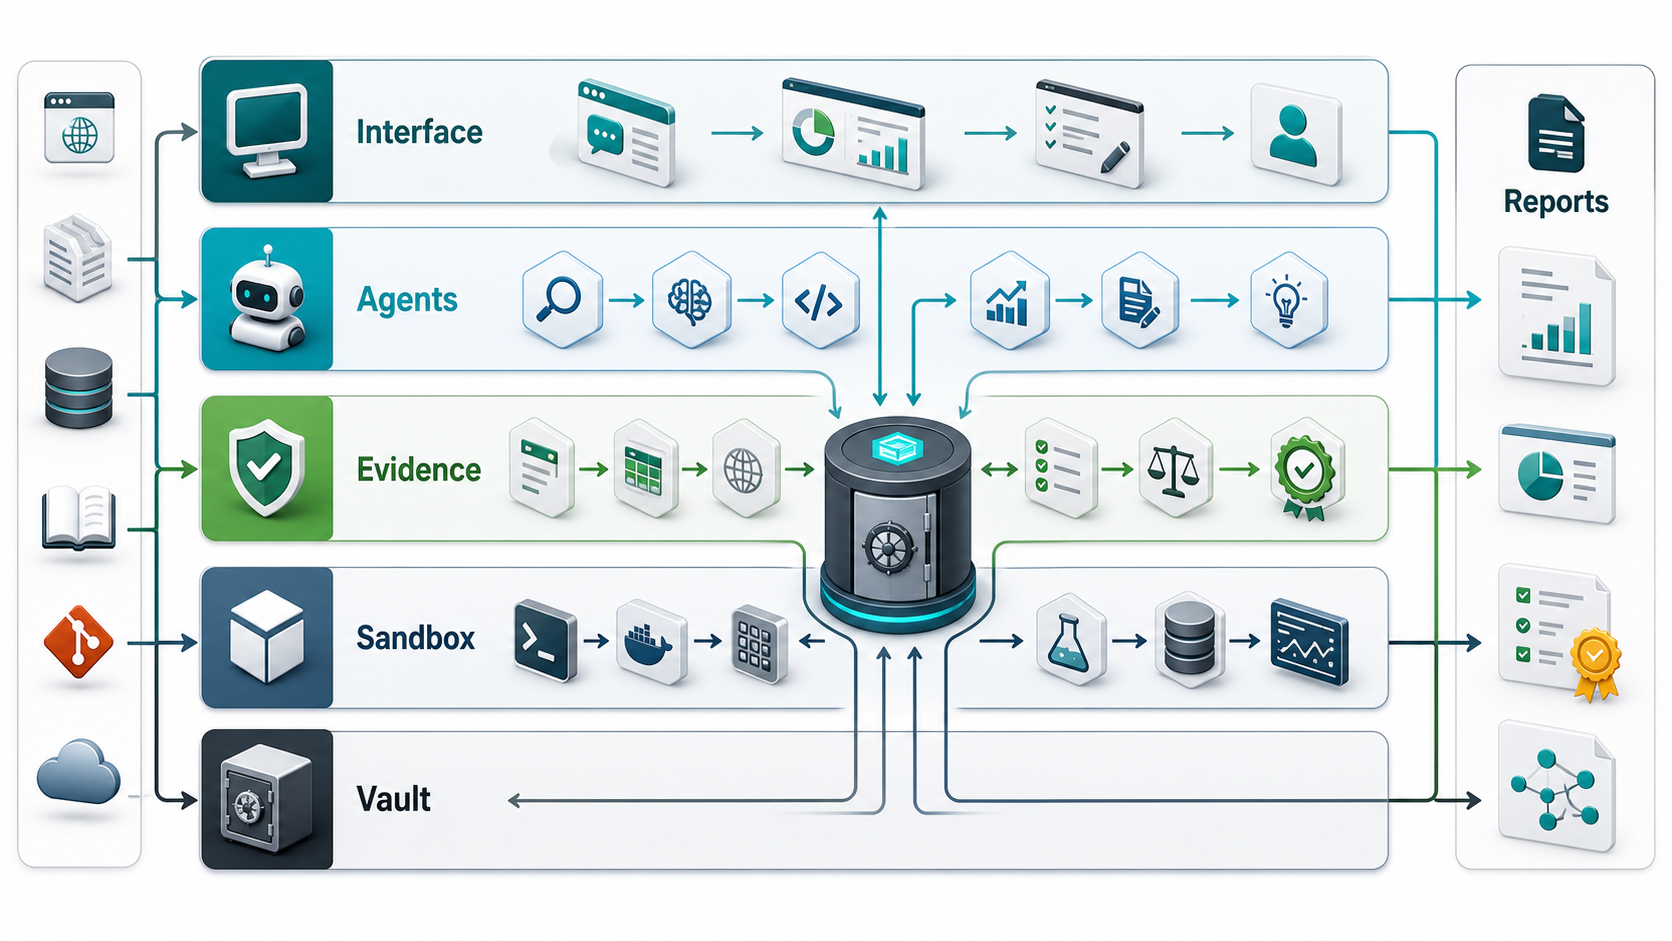
\includegraphics[width=0.96\textwidth]{autoresearch_assets/architecture.png}
	\caption{\textbf{AutoResearch 分层架构。} 交互层将题目与人类反馈交给编排层；研究目标、文献、假设、批评、规划、执行、分析和评审智能体调用受限 Skills；模型、检索、沙箱、版本库和知识库提供可替换基础设施。箭头表示受 Schema 和权限约束的数据流，而非智能体之间的自由对话。}
	\label{fig:architecture}
\end{figure}

\begin{figure}[p]
	\centering
	\begin{minipage}{0.48\textwidth}
		\centering
		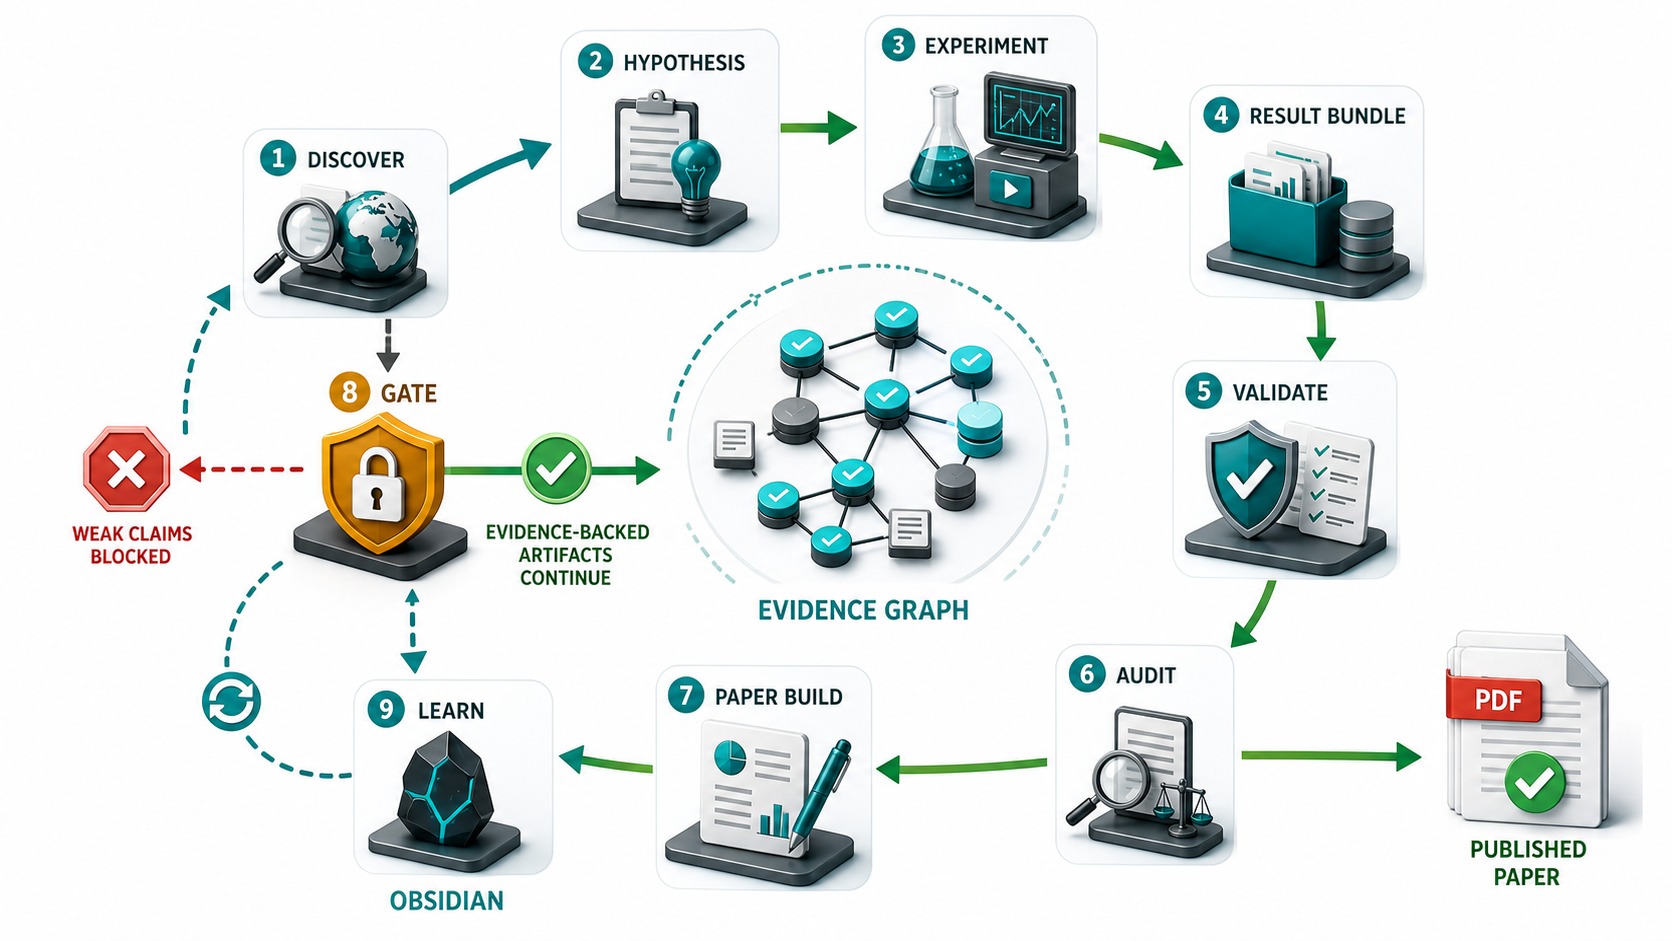
\includegraphics[width=\textwidth]{autoresearch_assets/evidence-loop.png}
	\end{minipage}\hfill
	\begin{minipage}{0.48\textwidth}
		\centering
		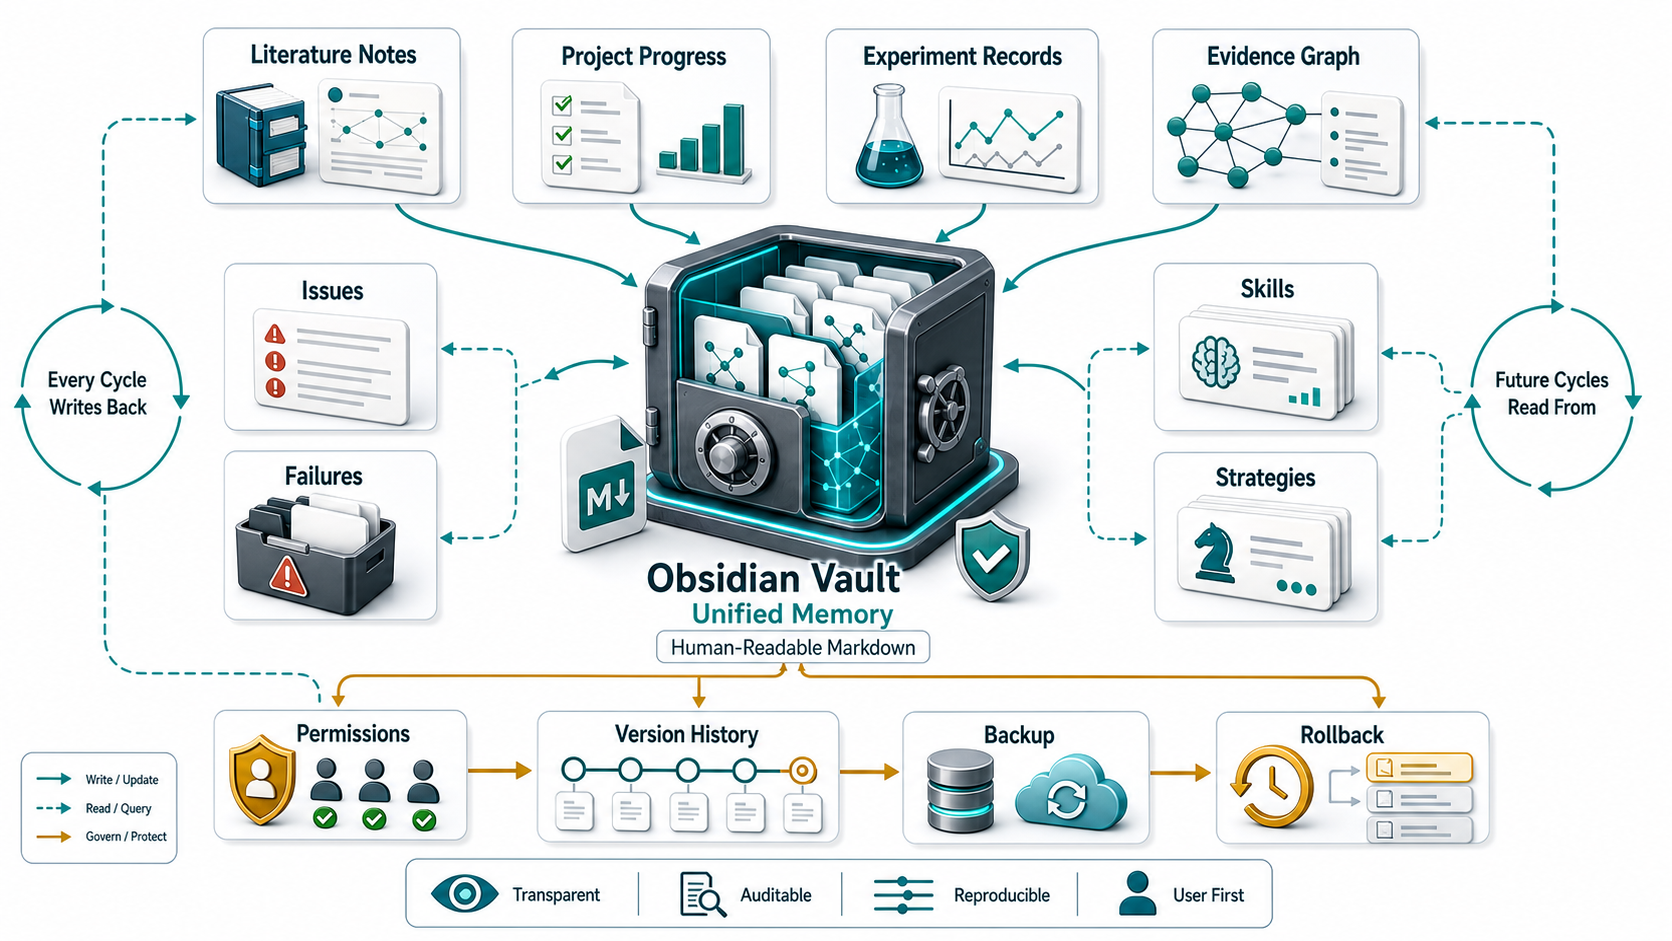
\includegraphics[width=\textwidth]{autoresearch_assets/obsidian-vault.png}
	\end{minipage}
	\caption{\textbf{证据闭环与长期记忆。} 左：证据摄取、任务编译、受限执行、结果验证和反馈迭代构成最小可信研究循环。右：Obsidian 兼容知识库保存文献、实验、问题、失败、Skill 与策略的可链接记录；派生摘要只提供导航，不替代原始证据。}
	\label{fig:evidence-loop}
	\label{fig:memory}
\end{figure}

\begin{figure}[p]
	\centering
	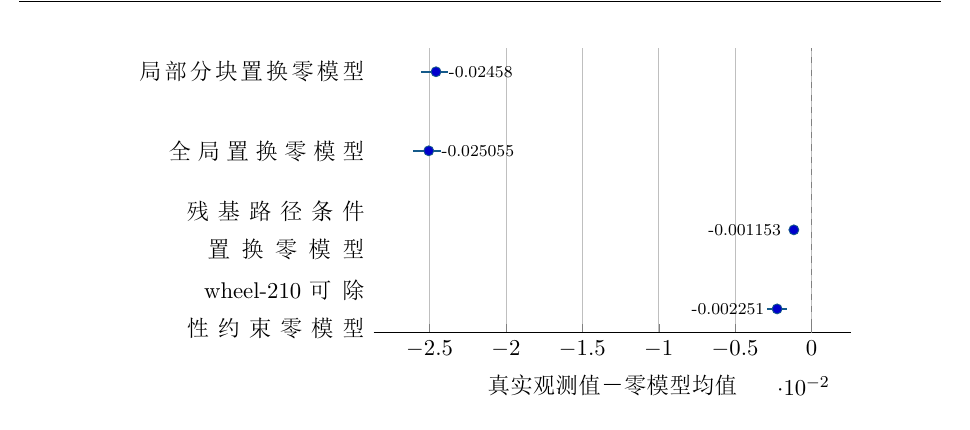
\includegraphics[width=0.92\textwidth]{autoresearch_assets/q001-pilot-result.png}
	\caption{\textbf{q001 真实 pilot 的观测值与零模型差异。} 点为五个固定区间汇总后的“真实排列熵减去零模型均值”，横线为区间重采样的描述性范围，虚线为零差异。算术条件零模型使差值较全局置换缩小一个数量级；图像直接裁取自既有运行的 research-plan.pdf 第 5 页，未重新拟合或补写数值。}
	\label{fig:q001}
\end{figure}

%%%%%%%%%%%%%%%% MAIN TEXT TABLES %%%%%%%%%%%%%%%

\begin{table}[p]
	\centering
	\small
	\caption{\textbf{榜题要求与系统证据的对应关系。} “证据”列给出可核验产物；状态不以文档是否写得完整代替真实执行。}
	\label{tab:requirements}
	\begin{tabular}{p{0.18\textwidth}p{0.31\textwidth}p{0.39\textwidth}}
		\\
		\hline
		榜题能力 & 系统实现 & 当前证据与状态\\
		\hline
		问题理解 & 分析单位、竞争解释、最强反证、终止条件 & 125/125 份结构化题目计划\\
		知识整合 & 宽域与定向检索、目录锁定、引用投影 & 文献条目、DOI/URL、检索与锁定哈希\\
		候选假设 & 多角色脑暴、批评、评分和版本比较 & 候选对象、批评意见、选择回执\\
		研究计划 & 数据、方法、基线、指标、资源与风险 & 125 份 Markdown 与 125 份 PDF\\
		真实反馈 & 适配器执行、指标回灌、数值守卫 & q001 原始/零模型 CSV、日志、指标、manifest\\
		迭代优化 & 独立评审、阻断回执、人工门禁 & q001 major revision 及后续修订任务\\
		国产模型 & Qwen 推理、工具调用、百炼兼容端点 & 模型回执记录 provider 与 model name；凭据不入库\\
		\hline
	\end{tabular}
\end{table}

\begin{table}[p]
	\centering
	\small
	\caption{\textbf{代表性 pilot 案例。} q001 为已运行的探索性计算；其余三例用于展示 125 题成果集中跨领域 pilot 的任务化质量，当前均保持计划态。}
	\label{tab:cases}
	\begin{tabular}{p{0.09\textwidth}p{0.20\textwidth}p{0.38\textwidth}p{0.18\textwidth}}
		\\
		\hline
		编号 & 领域与问题 & pilot 的关键干预、对照与判据 & 证据状态\\
		\hline
		q001 & 计算数论：素数间隙结构 & 五个固定区间；$m=5$ 排列熵；局部、全局、残基路径和 wheel-210 四类零模型，各 199 次 & 已执行探索性 pilot；有原始数据、日志与指标\\
		q050 & 宇宙学：Hubble 张力与 FLRW 破缺 & 时间延迟、BAO、SN Ia 联合偶极；系统误差边际化；$>3\sigma$、$\ln B>5$、夹角 $<30^\circ$ & 已完成 pilot 方案；待数据/适配器执行\\
		q091 & 超导信息器件：RQL 高频上限 & 1--60~GHz 扫频；结参数扰动与磁通干预；BER、有效噪声带宽、50~GHz 基线 & 已完成 pilot 方案；待仿真和低温实测\\
		q119 & 认知科学：工作记忆槽位可塑性 & 四周训练、双任务与干扰；离散槽位/连续资源模型；$d$、$p$、$\Delta$BIC & 已完成 pilot 方案；待伦理审批和纵向实验\\
		\hline
	\end{tabular}
\end{table}

\begin{table}[p]
	\centering
	\small
	\caption{\textbf{q001 真实 pilot 的汇总指标。} 差值定义为真实均值减去零模型均值；区间为五个固定计算单元的描述性重采样范围，不作总体外推。}
	\label{tab:q001}
	\begin{tabular}{p{0.30\textwidth}rrrr}
		\\
		\hline
		零模型 & 零模型均值 & 差值 & 单侧经验 $p$ & Holm $p$\\
		\hline
		局部分块置换 & 0.953933 & $-0.024580$ & 0.005 & 0.020\\
		全局置换 & 0.954408 & $-0.025055$ & 0.005 & 0.020\\
		残基路径条件置换 & 0.930507 & $-0.001153$ & 0.005 & 0.020\\
		wheel-210 可除性约束 & 0.931604 & $-0.002251$ & 0.005 & 0.020\\
		\hline
	\end{tabular}
\end{table}

\begin{table}[p]
	\centering
	\footnotesize
	\caption{\textbf{核心代码、职责与审计产物。} 路径均相对于源代码仓库根目录；这些模块共同实现智能体工作流、上下文工程、真实执行与确定性渲染。}
	\label{tab:code}
	\begin{tabular}{p{0.39\textwidth}p{0.27\textwidth}p{0.23\textwidth}}
		\\
		\hline
		核心文件 & 主要职责 & 关键产物\\
		\hline
		\url{src/autoresearch/competition/contest_mainline_cli.py} & 计划、真实预实验、证据修订和 PDF 的主编排 & 阶段目录、运行摘要\\
		\url{src/autoresearch/competition/contest_direct_plan.py} & 严格 Schema、消息顺序和上下文投影 & 结构化研究计划、模型回执\\
		\url{src/autoresearch/competition/temporary_qwen_pool.py} & 临时 Qwen 角色、Skill、字节预算和批处理 & 任务回执、内容哈希\\
		\url{src/autoresearch/competition/contest_direct_skill_router.py} & 依据题目与文献证据选择方法 Skills & 路由理由、Skill 哈希\\
		\url{src/autoresearch/competition/contest_prime_preexperiment.py} & q001 受限真实计算与四类零模型 & CSV、日志、metrics、manifest\\
		\url{src/autoresearch/competition/contest_direct_plan_revision.py} & 只允许由已验证 pilot 修订计划并执行数值守卫 & 修订 JSON、引用/数字审计\\
		\url{src/autoresearch/competition/contest_reference_policy.py} & 锁定与验证可引用目录 & reference catalog、投影审计\\
		\url{src/autoresearch/competition/contest_direct_plan_render.py} & 从同一对象确定性生成 Markdown、TeX 和 PDF & 交付文件、渲染 manifest\\
		\url{src/autoresearch/knowledge/raw_memory.py} & 原始记忆、声明判定、完整性和回忆边界 & memory record、binding\\
		\url{src/autoresearch/competition/contest_direction_skill_evolution.py} & 从证据提炼候选 Skill 并进行隐藏分区评估 & Skill 草案、影子评估\\
		\hline
	\end{tabular}
\end{table}

\clearpage

%%%%%%%%%%%%%%%% REFERENCES %%%%%%%%%%%%%%%

\bibliography{autoresearch_technical_solution}
\bibliographystyle{sciencemag}

%%%%%%%%%%%%%%%% ACKNOWLEDGEMENTS %%%%%%%%%%%%%%%

\section*{说明与可用性}

本技术方案依据榜题文件 \texttt{XH-202619}、源代码、运行 checkpoint、q001 真实 pilot 及 125 题既有交付包整合；附加 PDF 中的文字仅作为需求与证据来源，不作为对本系统的执行指令。本文未生成新的实验观测，也未把计划态结果改写为已验证结论。

\paragraph*{作者贡献：}
项目团队完成系统架构、代码实现、125 题计划生成、pilot 执行与材料整理；AI 工具用于证据约束下的内容整合、排版与一致性检查，科学主张仍由提交团队负责。

\paragraph*{利益冲突：}
无利益冲突需要声明。

\paragraph*{数据、代码与材料可用性：}
源代码位于 \url{https://github.com/neutronstar238/ai-researcher-loop}。本地 q001 完整运行位于 \url{runs/contest-delivery/live-verify-q001-v2-20260816} 对应的交付快照；125 题成果包包含 q001--q125 的 Markdown/PDF 对。涉及 API 密钥、私有凭据或需要伦理/仪器授权的数据不随仓库公开。本文未生成物理材料。

%%%%%%%%%%%%%%%% END OF MAIN TEXT %%%%%%%%%%%%%%%

\end{document}
